\documentclass[11pt]{article}

\usepackage[margin=0.80in]{geometry}
\usepackage[T1]{fontenc}
\usepackage{newtxtext,newtxmath}
\usepackage{amsmath,amssymb}
\usepackage{booktabs,array,tabularx}
\usepackage{enumitem}
\usepackage{siunitx}
\usepackage{tikz}
\usepackage{fancyhdr}
\usepackage[hidelinks]{hyperref}

\setlength{\parindent}{0pt}
\setlength{\parskip}{5pt}
\setlist{nosep,leftmargin=1.6em}
\sisetup{detect-all,per-mode=symbol}

\pagestyle{fancy}
\fancyhf{}
\lhead{MIE 446: Aerospace Structures}
\rhead{Homework 1}
\cfoot{\thepage}
\renewcommand{\headrulewidth}{0.4pt}

\newcommand{\X}{\overline{x}}
\newcommand{\Yu}{\overline{y}_u}
\newcommand{\Yl}{\overline{y}_l}
\newcommand{\Yc}{\overline{y}_c}
\newcommand{\Yt}{\overline{y}_t}
\newcommand{\Cpu}{C_{p,u}}
\newcommand{\Cpl}{C_{p,l}}

\begin{document}

{\LARGE\bfseries Homework 1: Surface Pressure, Lift, and Pressure Drag}\par
\vspace{2pt}
{\large NACA 2412 at $\alpha=5^{\circ}$}\par
\vspace{6pt}
\hrule
\vspace{8pt}

\begin{tabularx}{\textwidth}{@{}X X@{}}
Name: \hrulefill & UMass ID: \hrulefill\\[7pt]
Due: \hrulefill & Section: \hrulefill
\end{tabularx}

\section*{Purpose}
In this homework you will compute the two-dimensional aerodynamic force produced by a pressure distribution on a NACA 2412 airfoil. In Question 1, the geometry and pressure are continuous functions and you will evaluate surface integrals. In Question 2, the same flight condition is represented by tabulated data and you will replace the integrals by finite differences and panel sums.

\begin{center}
\fbox{\parbox{0.94\textwidth}{\textbf{Model statement.} The supplied pressure distribution is a calibrated instructional surrogate for attached flow over a NACA 2412 section at $\alpha=5^{\circ}$. It is designed to reproduce a physically reasonable suction peak and a lift coefficient near the historical NACA 2412 trend. It is \emph{not} presented as pressure-tap measurement data or as a universal pressure law.}}
\end{center}

\section*{Given conditions and conventions}
\begin{center}
\begin{tabular}{ll@{\qquad}ll}
\toprule
Quantity & Value & Quantity & Value\\
\midrule
Airfoil & NACA 2412 & Angle of attack & $\alpha=5.0^{\circ}$\\
Chord & $c=\SI{0.500}{m}$ & Reference span & $b=\SI{1.000}{m}$\\
Freestream speed & $V_\infty=\SI{30.0}{m/s}$ & Density & $\rho_\infty=\SI{1.225}{kg/m^3}$\\
Static pressure & $p_\infty=\SI{101325}{Pa}$ & Dynamic pressure & $q_\infty=\tfrac12\rho_\infty V_\infty^2$\\
\bottomrule
\end{tabular}
\end{center}

Let $\X=x/c$ and $\overline y=y/c$. The $x$-axis points from the leading edge toward the trailing edge; the positive $y$-axis points upward. Pressure coefficient is
\begin{equation}
C_p=\frac{p-p_\infty}{q_\infty}.
\end{equation}
The pressure resultant is first resolved into a chord-normal coefficient $C_N$ and a chord-axial coefficient $C_A$. Positive $C_A$ points from leading edge to trailing edge. Lift and pressure drag are then obtained by rotation into wind axes:
\begin{align}
C_L &= C_N\cos\alpha-C_A\sin\alpha,\\
C_{D,p} &= C_N\sin\alpha+C_A\cos\alpha.
\end{align}

\begin{center}
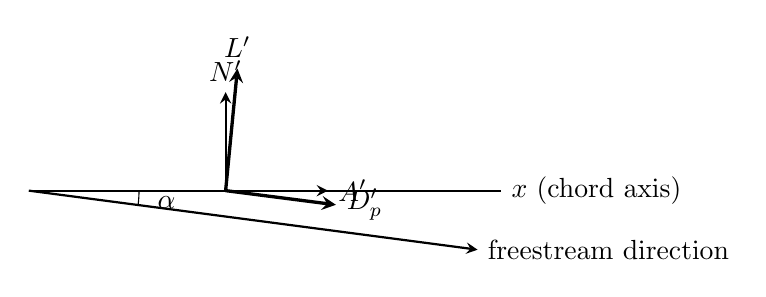
\begin{tikzpicture}[scale=1.0,>=stealth]
  \draw[thick] (0,0) -- (6,0) node[right] {$x$ (chord axis)};
  \draw[thick,->] (0,0) -- (5.7,-0.75) node[right] {freestream direction};
  \draw[->,thick] (2.5,0) -- (2.5,1.25) node[above] {$N'$};
  \draw[->,thick] (2.5,0) -- (3.8,0) node[right] {$A'$};
  \draw[->,very thick] (2.5,0) -- (2.65,1.55) node[above] {$L'$};
  \draw[->,very thick] (2.5,0) -- (3.9,-0.18) node[right] {$D_p'$};
  \draw (1.4,0) arc[start angle=0,end angle=-7.5,radius=1.4];
  \node at (1.75,-0.15) {$\alpha$};
\end{tikzpicture}
\end{center}

Only pressure forces are included. Therefore $C_{D,p}$ is \textbf{pressure drag}, not total viscous drag; skin-friction drag cannot be recovered from the supplied pressure data.

\section*{NACA 2412 geometry used in both questions}
For NACA 2412,
\[
m=0.02,\qquad p=0.40,\qquad t=0.12.
\]
The nondimensional mean camber line is
\begin{equation}
\Yc(\X)=
\begin{cases}
\dfrac{m}{p^2}\left(2p\X-\X^2\right), & 0\le \X\le p,\\[6pt]
\dfrac{m}{(1-p)^2}\left[(1-2p)+2p\X-\X^2\right], & p<\X\le1,
\end{cases}
\end{equation}
and the closed-trailing-edge thickness distribution is
\begin{equation}
\Yt(\X)=5t\left(0.2969\sqrt{\X}-0.1260\X-0.3516\X^2+0.2843\X^3-0.1036\X^4\right).
\end{equation}
Use the common-$x$ approximation
\begin{equation}
\Yu=\Yc+\Yt,\qquad \Yl=\Yc-\Yt.
\end{equation}
The slopes needed in the force integral are
\begin{equation}
\frac{d\Yu}{d\X}=\frac{d\Yc}{d\X}+\frac{d\Yt}{d\X},\qquad
\frac{d\Yl}{d\X}=\frac{d\Yc}{d\X}-\frac{d\Yt}{d\X},
\end{equation}
where
\begin{equation}
\frac{d\Yc}{d\X}=
\begin{cases}
\dfrac{2m}{p^2}(p-\X), & 0\le \X\le p,\\[6pt]
\dfrac{2m}{(1-p)^2}(p-\X), & p<\X\le1,
\end{cases}
\end{equation}
and
\begin{equation}
\frac{d\Yt}{d\X}=5t\left(\frac{0.2969}{2\sqrt{\X}}-0.1260-0.7032\X+0.8529\X^2-0.4144\X^3\right).
\end{equation}

\section*{Question 1 — Continuous surface integration \hfill [45 points]}
Define the following smooth loading model on $0\le\X\le1$:
\begin{align}
C_0(\X) &= (1-\X)\left[e^{-\X/0.010}+0.20\left(1-e^{-\X/0.020}\right)\right],\\
\Delta C_p(\X) &= 0.721896\,
\frac{\left(1-e^{-\X/0.010}\right)(1-\X)}{\sqrt{\X+0.020}},\\
\Cpu(\X) &= C_0(\X)-0.80\,\Delta C_p(\X),\\
\Cpl(\X) &= C_0(\X)+0.20\,\Delta C_p(\X).
\end{align}
The corresponding dimensional pressures are
\begin{equation}
p_u=p_\infty+q_\infty\Cpu,\qquad
p_l=p_\infty+q_\infty\Cpl.
\end{equation}

Complete the following tasks.
\begin{enumerate}[label=\textbf{1\alph*.}]
  \item Decode the four digits of NACA 2412. Calculate $q_\infty$ and state its units.
  \item Plot $\Yu$ and $\Yl$ on equal axes. On a separate graph, plot $\Cpu$ and $\Cpl$ against $\X$ using the aerodynamic convention in which the $C_p$ axis is inverted. Identify the leading-edge suction region and the pressure difference that produces positive lift.
  \item Starting from the pressure force on each surface, show that the common-$x$ model gives
  \begin{align}
  C_N &= \int_0^1(\Cpl-\Cpu)\,d\X,\\
  C_A &= \int_0^1\left(\Cpu\frac{d\Yu}{d\X}-\Cpl\frac{d\Yl}{d\X}\right)d\X.
  \end{align}
  State the sign convention used for $C_A$.
  \item Evaluate $C_N$ and $C_A$ numerically. The thickness slope contains $1/\sqrt{\X}$ at the leading edge, but the integral is finite. Use adaptive quadrature, begin at a documented small positive value, or use the substitution $\X=s^2$. State your method and demonstrate numerical convergence using two tolerances or two discretizations.
  \item Calculate $C_L$, $C_{D,p}$, and the forces per unit span
  \begin{equation}
  L'=q_\infty c C_L,\qquad D_p'=q_\infty c C_{D,p}.
  \end{equation}
  Report coefficients to four significant figures and forces to an appropriate precision.
  \item Give two physical checks on your answer. At minimum, discuss the signs and relative magnitudes of lift and pressure drag and explain why this calculation cannot produce total viscous drag.
\end{enumerate}

\section*{Question 2 — Tabulated data and discrete panel sums \hfill [45 points]}
Download the companion workbook \texttt{MIE446\_HW1\_NACA2412\_Data.xlsx}. The \texttt{Data} sheet contains 101 stations from $\X=0$ to $1$ and the five supplied quantities $\X$, $\Yu$, $\Yl$, $p_u$, and $p_l$. Do not replace the supplied values.

\begin{enumerate}[label=\textbf{2\alph*.}]
  \item In new columns, calculate $\Cpu$ and $\Cpl$ from the tabulated dimensional pressures.
  \item Calculate $d\Yu/d\X$ and $d\Yl/d\X$ at every station. For interior points use the centered difference
  \begin{equation}
  \left(\frac{d\overline y}{d\X}\right)_i\approx
  \frac{\overline y_{i+1}-\overline y_{i-1}}{\X_{i+1}-\X_{i-1}},
  \end{equation}
  and use one-sided differences at the first and last stations. Retain the leading-edge values; do not hide them because they are large.
  \item Form the pointwise integrands
  \begin{equation}
  I_{N,i}=C_{p,l,i}-C_{p,u,i},\qquad
  I_{A,i}=C_{p,u,i}\left(\frac{d\Yu}{d\X}\right)_i-C_{p,l,i}\left(\frac{d\Yl}{d\X}\right)_i.
  \end{equation}
  Use the trapezoidal rule over the 100 intervals:
  \begin{equation}
  C_N\approx\sum_{i=1}^{100}\frac{I_{N,i}+I_{N,i+1}}{2}\,\Delta\X_i,
  \qquad
  C_A\approx\sum_{i=1}^{100}\frac{I_{A,i}+I_{A,i+1}}{2}\,\Delta\X_i.
  \end{equation}
  Keep each interval contribution visible in the workbook.
  \item Independently check the axial result with the direct panel line integral
  \begin{equation}
  \Delta C_{A,i}=\overline C_{p,u,i}\left(\Yu_{i+1}-\Yu_i\right)
  -\overline C_{p,l,i}\left(\Yl_{i+1}-\Yl_i\right),
  \end{equation}
  where $\overline C_{p,u,i}=(C_{p,u,i}+C_{p,u,i+1})/2$, and similarly for the lower surface. Sum all 100 panel contributions. Explain why this form avoids dividing by a small $\Delta\X$.
  \item Rotate the discrete $C_N$ and $C_A$ into $C_L$ and $C_{D,p}$, then calculate $L'$ and $D_p'$. Compare Question 2 with Question 1 using
  \begin{equation}
  \%\text{ difference}=100\left|\frac{\text{discrete}-\text{continuous}}{\text{continuous}}\right|.
  \end{equation}
  Comment separately on the lift difference and pressure-drag difference. Pressure drag is obtained by cancellation of two larger terms and is therefore more sensitive to discretization.
  \item Create two clear Excel charts: airfoil geometry and inverted-$C_p$ distribution. Label axes and identify upper and lower surfaces.
\end{enumerate}

\section*{Submission and engineering communication \hfill [10 points]}
Submit the following through Canvas:
\begin{itemize}
  \item one PDF containing derivations, figures, results, units, and your comparison;
  \item the completed Excel workbook with formulas visible and traceable;
  \item one summary slide containing the method, final values, and one independent check;
  \item a brief AI-use disclosure.
\end{itemize}

\textbf{AI statement.} AI tools may be used for syntax help, debugging, plotting, and checking intermediate work. You remain responsible for the derivation, spreadsheet formulas, physical interpretation, and verification. Briefly disclose what tool was used, for what purpose, and what independent check you performed. ``The AI produced this answer'' is not a verification method.

\section*{Grading guide}
\begin{center}
\begin{tabularx}{\textwidth}{X r}
\toprule
Criterion & Points\\
\midrule
Question 1: geometry, pressure interpretation, and force derivation & 18\\
Question 1: integration, convergence, coefficients, forces, and checks & 27\\
Question 2: spreadsheet organization, $C_p$, slopes, and integrands & 18\\
Question 2: trapezoidal sum, direct-panel check, rotation, and comparison & 27\\
Figures, units, summary slide, and AI disclosure & 10\\
\midrule
Total & 100\\
\bottomrule
\end{tabularx}
\end{center}

\section*{References}
\begin{enumerate}
  \item E.~N. Jacobs, K.~E. Ward, and R.~M. Pinkerton, \emph{The Characteristics of 78 Related Airfoil Sections from Tests in the Variable-Density Wind Tunnel}, NACA Report 460. \url{https://ntrs.nasa.gov/citations/19930091108}
  \item NASA OpenVSP Ground School, ``NACA 4-Series Airfoil.'' \url{https://www.nasa.gov/reference/openvsp-cross-sections/}
  \item NASA Glenn Research Center, ``Lift Equation.'' \url{https://www1.grc.nasa.gov/beginners-guide-to-aeronautics/lift-equation/}
\end{enumerate}

% INSTRUCTOR CHECK VALUES — REMOVE BEFORE STUDENT RELEASE:
% High-resolution continuous reference for the stated model:
% q_inf = 551.25 Pa; C_N = 0.742000; C_A = -0.0558168;
% C_L = 0.744041; C_D,p = 0.00906515;
% L' = 205.08 N/m; D_p' = 2.499 N/m.
% With the 101-point uniform dataset and the stated finite differences:
% C_N ≈ 0.737895; C_A ≈ -0.0587520;
% C_L ≈ 0.740207; C_D,p ≈ 0.00578333;
% L' ≈ 204.02 N/m; D_p' ≈ 1.594 N/m.

\end{document}
